% Guidance - 3 pages
% A technical description of the problem in terms of the requirements given,
% expanded into a discussion and highlighting likely implied technical aspects
% and challenges that need/needed to be tackled
\section{Description of Problem and Requirements}
The Embedded Systems Project consisted of two main sections: a group solution 
to a predetermined problem, and an individual extension to the group's work, 
left up to each person to determine. Both sections of the project involved 
embedded systems software development in the C programming language. 
\par\bigskip\noindent
The target platform of the development is an ARM-based microcontroller, 
situated on a board of peripheral accessories. The microcontroller consists of 
an interface board coupled with the ARM cortex-M3 based LPC1768, providing easy 
interaction via USB cable to transfer binaries, and simplifying the process of 
serial communication [how-mbed-works].
\par\bigskip\noindent
The MBED board is sat on a board of peripheral accessories, as pictured below. 
\par\bigskip
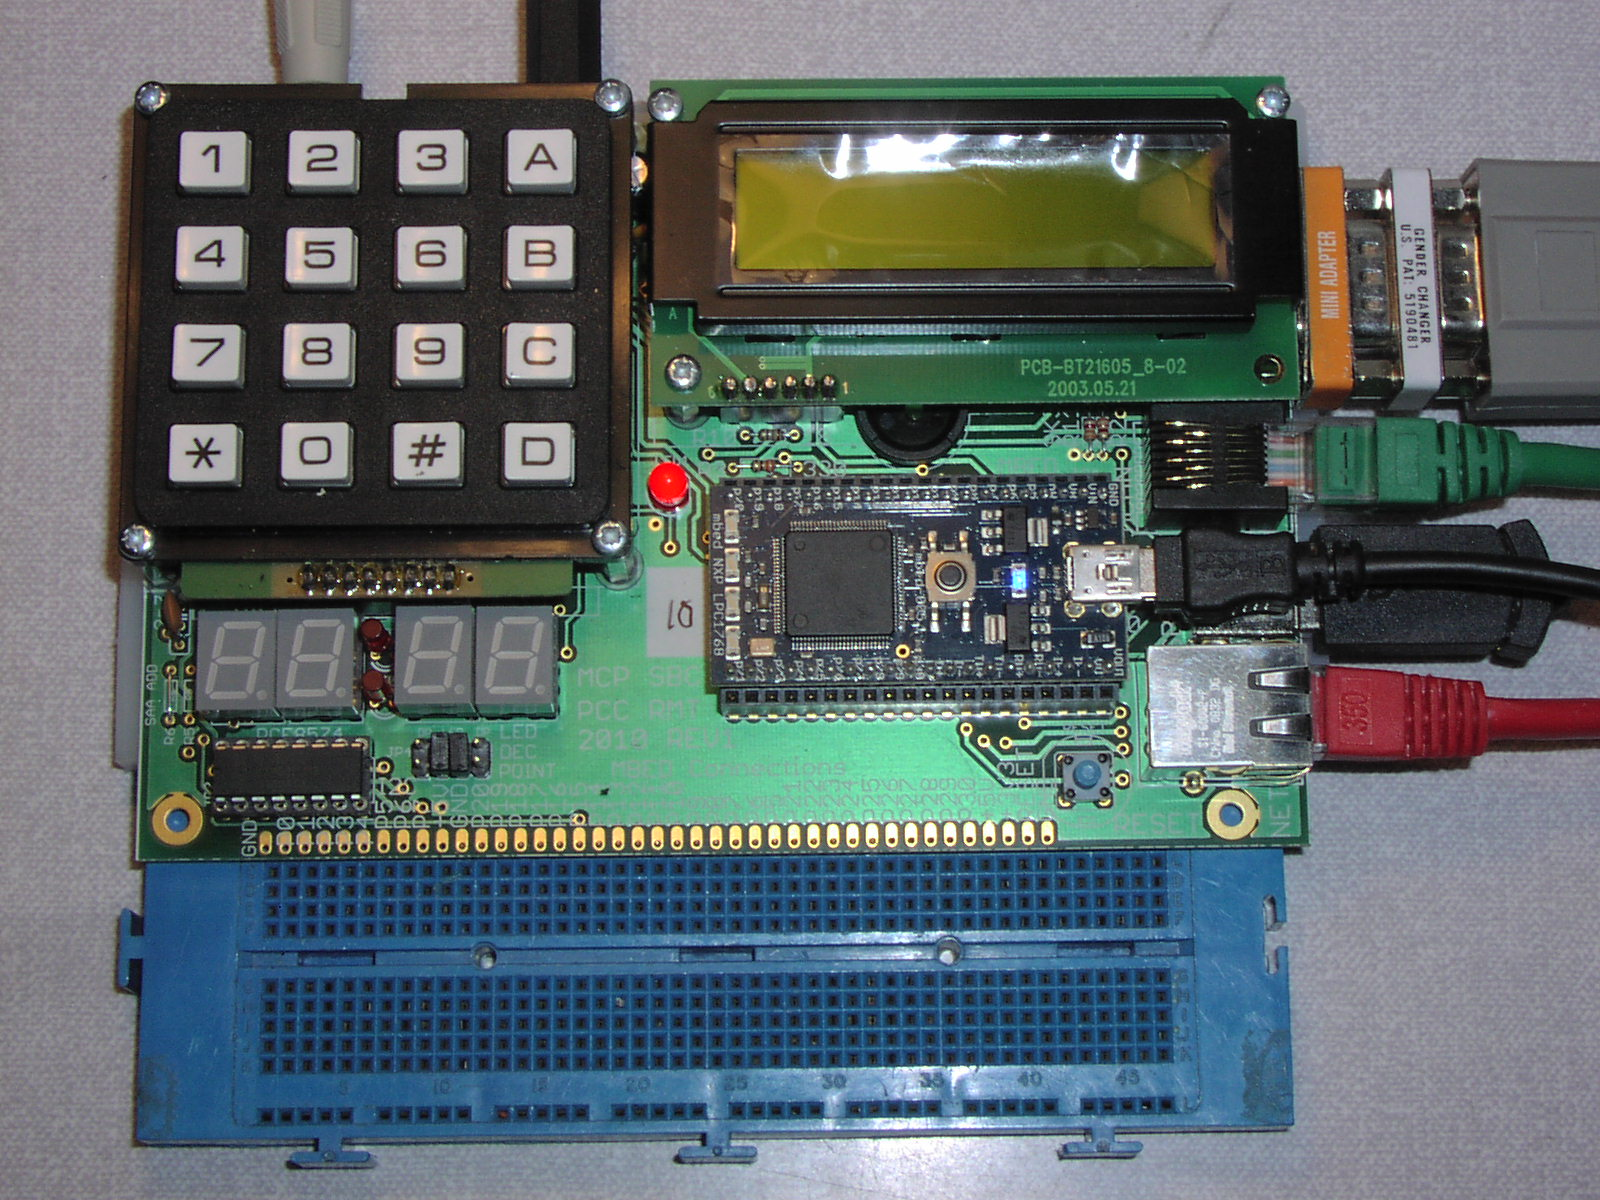
\includegraphics[width=0.80\textwidth]{./mbed_board}
\par\bigskip\noindent
The board contains multiple accessories that the MBED board can interface with 
in various ways to fulfil the requirements, and allowing many options for 
individual extensions. The accessories on the board include: a 16 key keyboard, 
a 16 by 2 line LCD, four seven segment displays, a micro SD slot, a USB host 
connection, CAN bus connecter, audio in and out jacks, a TCP/IP connection, as 
well as off board connections to users hardware. 

\par\bigskip\noindent
The group task consisted of multiple different challenges, with the concept
that the MBED board would continually receive CAN packets, filter out those 
that do not match a user selectable id, decode the CAN packets, and play notes 
corresponding to the frequency, volume, and duration that were specified from 
the CAN transmissions. In addition the user must be able to view useful 
information, select the channel id, and adjust the volume. 

\par\bigskip\noindent
In addition there was an individual component. This did not have to match any 
specification, and was instead left up to each person to decide on their own 
extension to the group project. For my individual extension, I implemented a 
Linux shell style user interface. This allows user to interact with the device 
by typing commands into a terminal on their computer, effectively adding an 
additional element of user control that is more intuitive and responsive than 
using the 16 digit keypad from the MBED board.

\par\bigskip\noindent
For our group solution, the specification was broken down into three separate 
areas, allowing us to focus our expertise and interests on what suited us best.
The breakdown of the three sections was as follows: The receiving and 
decoding of CAN packets (CAN bus), generation of audio samples corresponding to 
frequency, duration and volume (Audio), and the ability for the user to 
interact with the device in order to adjust settings (User Interface). 

\section{Discussion of Technical Aspects and Challenges}

As previously mentioned, my group deconstructed the specification into three 
main areas of technical challenge. The first of these challenging areas regarded 
the receiving of data from the CAN bus, and the decoding of the packets received
to extract their content. As the CAN packets are not arriving at regularly 
timed intervals, the solution to this problem is required to be interrupt based. 
However, due to the nature of the CAN packets, a very large number can arrive in 
a comparatively short space of time. This therefore requires a highly optimised 
solution, in order to prevent packets either being missed, or race conditions 
within the interrupt handler from occurring. 
\par\bigskip\noindent
The second technical challenge of the project is the generation of audio tones 
corresponding to frequency, duration and volume levels as specified by the CAN 
packets. The CAN packets do not contain information detailing what each note 
should sound like. As a result, all musical notes need to be generated from 
first principals, for example using a look up table detailing values for a note 
at each moment in time. In combination, to make the notes sound more realistic, 
each note must go through at least three stages. The first of these stages 
defines the initial playing of a note, plucking a string or pressing a key. This
 is known as 'attack'. The second stage corresponds to the continual noise made 
from the note until it is stopped and is known as 'sustain'. The final stage 
details the note as it dies down and stops and is known as 'release'. This 
presents additional problems as each note requires multiple states, and needs to 
be tracked in its progress through each. 
Furthermore, it may be an additional desire to play more than one note at any 
one moment in time. This requires synthesis of multiple different notes in order 
to produce an appropriate output. The mathematics of this can be expensive to 
compute, and furthermore, an increase in the number of notes can drastically 
increase the processing time. A delay in the output of the notes can lead to 
a strange sounding finished product, so the efficiency of any synthesis 
calculations are paramount to the end product. 
\par\bigskip\noindent
The third technical challenge that can be presented is the user's control over 
the device. The specification determines that the user must be able to control 
the volume of the output, alter which channel of notes is being played, 
and view useful information on the MBED board. This requires a level of
interaction, most likely via the 16 digit keypad on the device, however this 
could be via alternate input methods, such as a computer keyboard. The user's 
interaction with either device once again may not be continual, but may either 
be polled, at the cost of system resources, or interrupt based. Further 
challenges are presented as any possible user input must be stored on the device, 
parsed on command, and then the desired command must be executed without any 
significant effect on the audio output. Furthermore, the challenge is made 
increasingly difficult by the required ability to interface with the entire 
project: the audio synthesis code and the CAN bus code must be fully understood 
in order to be manipulated through the user's input. 
